% Template for ICIP-2015 paper; to be used with:
%          spconf.sty  - ICASSP/ICIP LaTeX style file, and
%          IEEEbib.bst - IEEE bibliography style file.
% --------------------------------------------------------------------------
\documentclass{article}
\usepackage{spconf,amsmath,graphicx}
\usepackage[utf8]{inputenc} % Suporte para acentuação sem necessidade dos comandos especiais.
\usepackage{amsmath,epsfig}
\usepackage[portuguese,algoruled,longend]{algorithm2e}
\usepackage{multirow}
\usepackage{MnSymbol}
\usepackage{wasysym}
\usepackage[table,xcdraw]{xcolor}
\usepackage[brazilian]{babel}
\usepackage{url}
\usepackage{float}
\usepackage{enumerate}
\usepackage{multicol}
\usepackage[numbered,framed]{matlab-prettifier}
\usepackage{soul,framed} %,caption
\usepackage{steinmetz}
\usepackage{subfigure}
\usepackage{lipsum}% for dummy text
\colorlet{shadecolor}{yellow}

% Template includegraphics
% \begin{figure}[H]
% 	\begin{center}
% 		\label{fig:11}
% 		\includegraphics[width=2.5in]{Figures/S02_Grafico_Ajustado.png}
% 		\caption{Gráficos da Situação 03 Ajustados}
% 	\end{center}
% \end{figure}  

% Example definitions.
% -------------------
\def\x{{\mathbf x}}
\def\L{{\cal L}}
% Title.
% ------
\title{Prova 2 - Processamento de Sinais Biológicos}
%
% Single address.
% ---------------
\name{Davi de Alencar Mendes (\url{dmendes@aluno.unb.br}) - 16/0026415}
\address{Engenharia Eletrônica, UnB-FGA, Brasília, Brasil}

\begin{document}
\onecolumn
\maketitle

% --------------------------------------------------------------------------
\section{Questão 1 - Compactação de Energia em Transformadas Wavelet 2D}
\subsection*{A - Decomposição separável em 3,4 e 5 níveis}
Para a decomposição foram escolhidos os filtros: \textit{db3}, \textit{sym4} e \textit{bior3.1}. Cada um destes apresenta propriedades diferentes em especial quanto a fase e é notório também o uso de wavelets do tipo biortogonal em aplicações de compressão de imagens com transformadas.

A eficácia de uma transformada depende da compactação de energia provida. Uma maneira de mensurar a compactação de energia é mostrada em \cite{jayant}, trata-se de uma medida para uma transformada ortonormal por meio da divisão entre a média aritmética da variância dos coeficientes pela sua média geométrica. Essa razão é conhecida como \textit{Transform Coding Gain - $G_{TC}$}:

Incialmente, acreditoque a imagem 1 possa ser melhor representada já que qualitativamente apresenta contornos menos complexos que a imagem 2. Entretanto, a análise do $G_{TC}$ revela que há maior ganho para a imagem 2.

\begin{equation}
	G_{TC} = \frac{\frac{1}{N}\sum_{i=0}^{N-1} \sigma_i^2}{(\prod_{i=0}^{N-1}\sigma_i)^{1/N}}
\end{equation}

As figuras a seguir mostram as decomposições obtidas para a imagem 1 (corte com olhos) e imagem 2 (corte cerebral).
\begin{figure}[H]
	\begin{center}
		\label{fig:1_db3}
		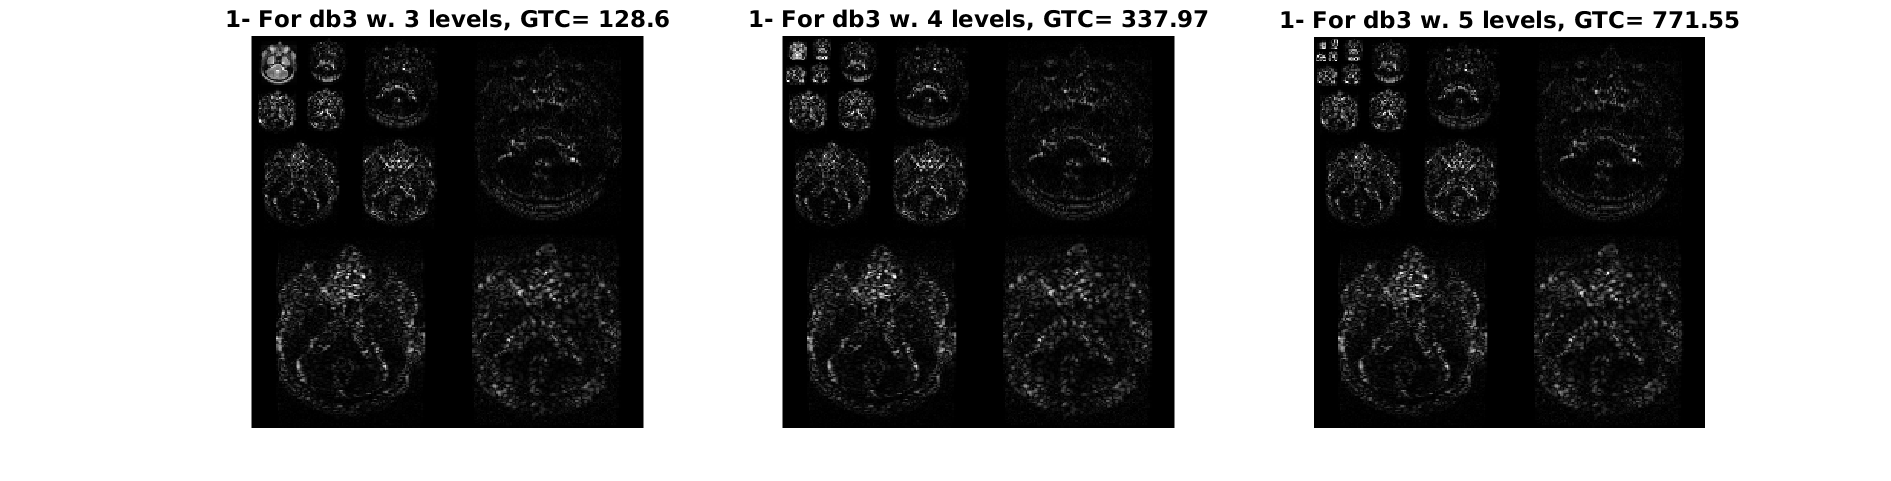
\includegraphics[scale=0.55]{../1_db3.png}
		\caption{Decomposição usando db3 para a imagem 1}
	\end{center}
\end{figure}  

\begin{figure}[H]
	\begin{center}
		\label{fig:1_sym4}
		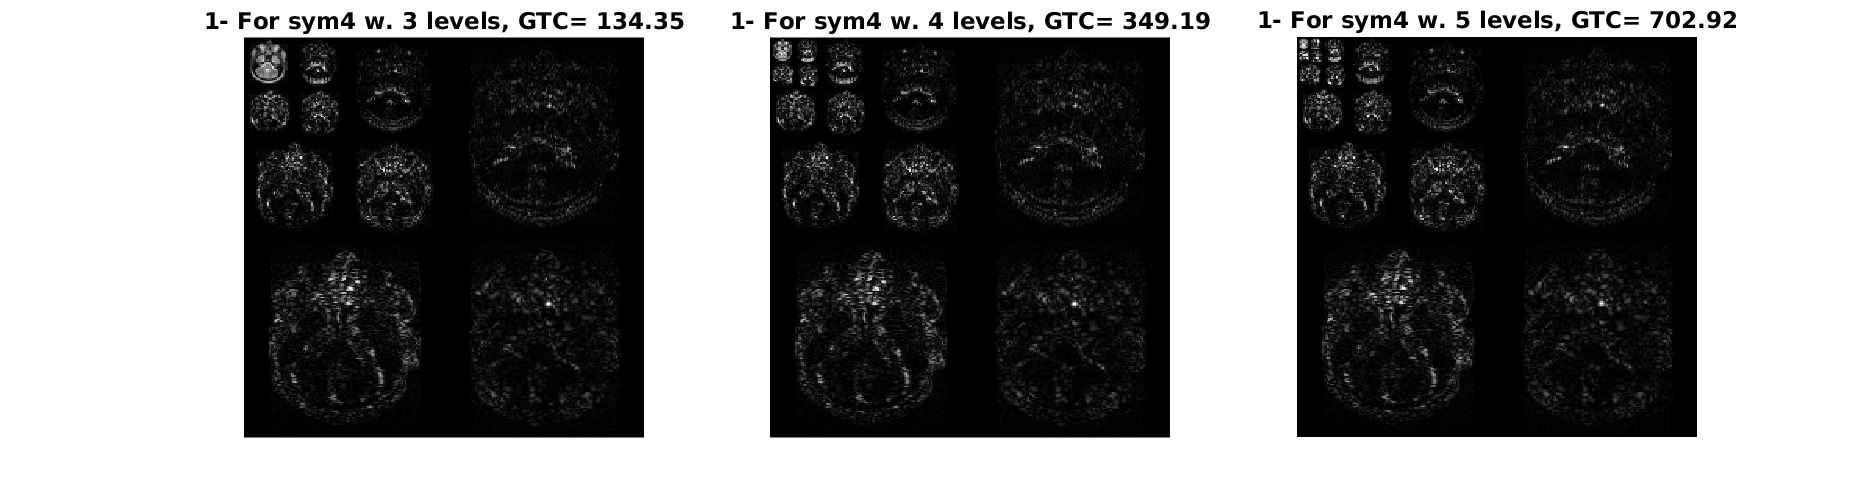
\includegraphics[scale=0.55]{../1_sym4.png}
		\caption{Decomposição usando sym4 para a imagem 1}
	\end{center}
\end{figure}  

\begin{figure}[H]
	\begin{center}
		\label{fig:1_bior3.1}
		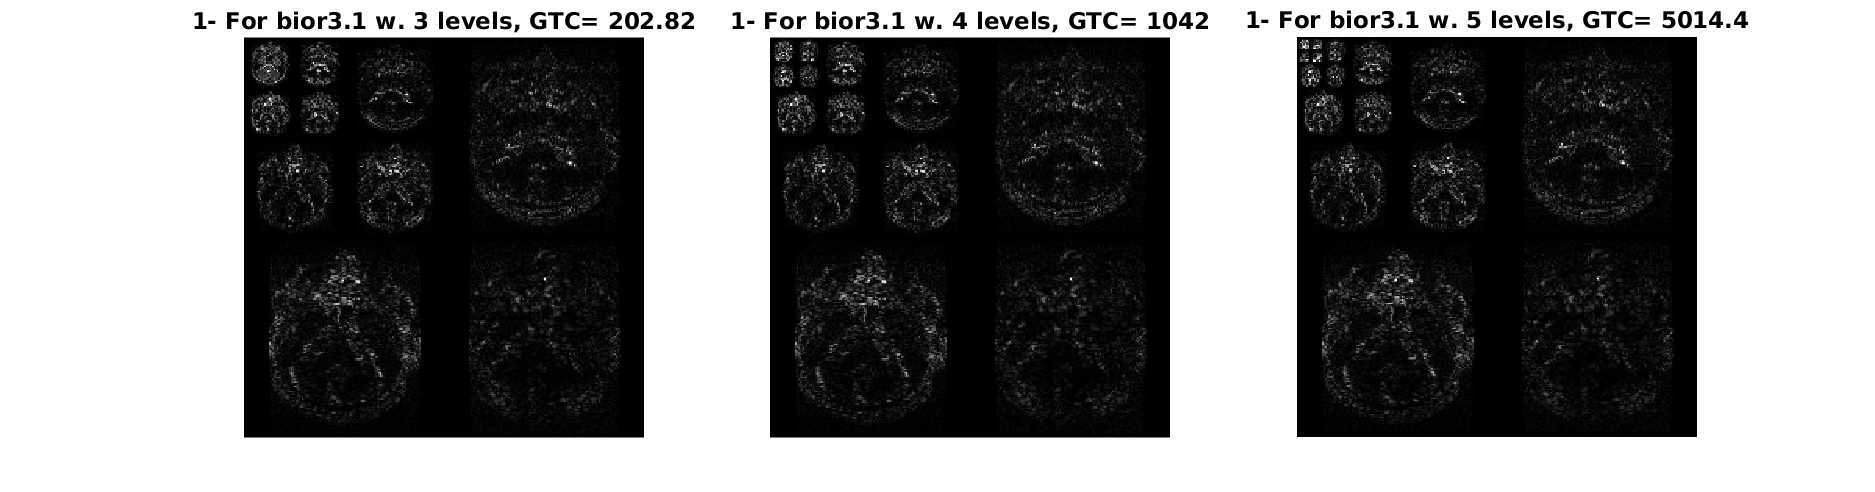
\includegraphics[scale=0.55]{../1_bior31.png}
		\caption{Decomposição usando bior3.1 para a imagem 1}
	\end{center}
\end{figure}  

\begin{figure}[H]
	\begin{center}
		\label{fig:2_db3}
		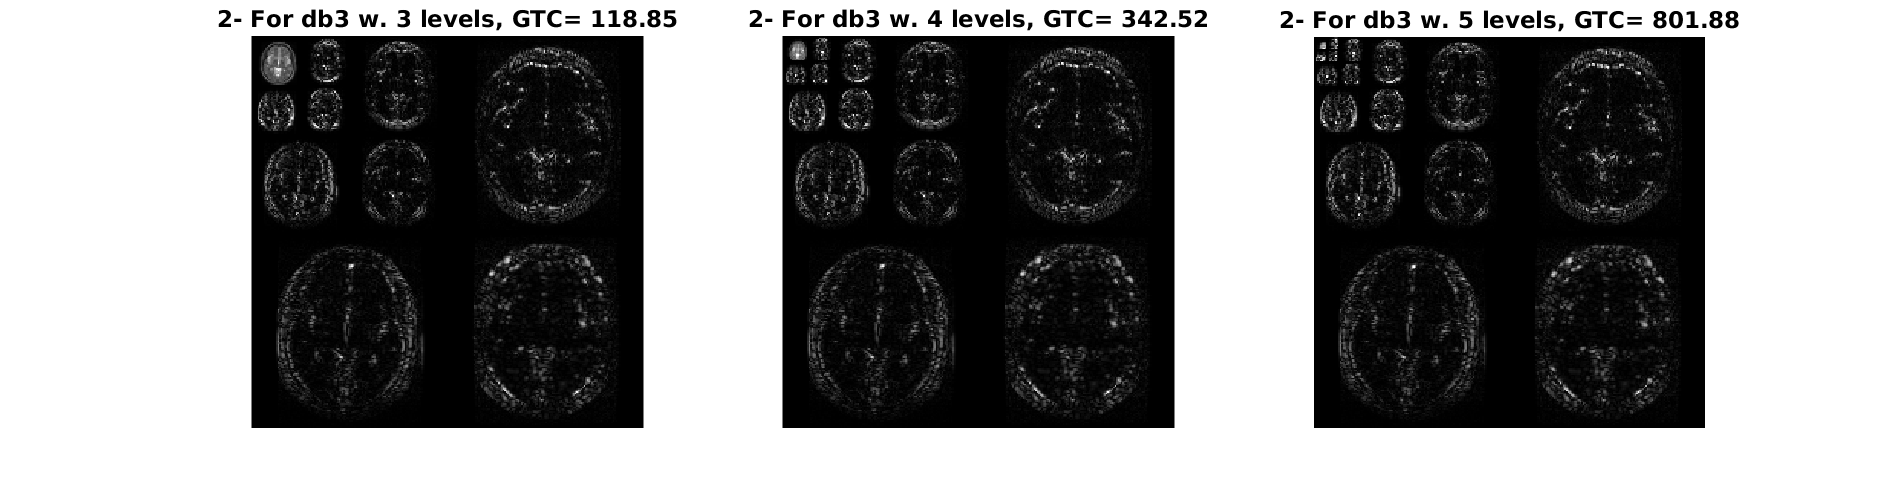
\includegraphics[scale=0.55]{../2_db3.png}
		\caption{Decomposição usando db3 para a imagem 2}
	\end{center}
\end{figure}  

\begin{figure}[H]
	\begin{center}
		\label{fig:2_sym4}
		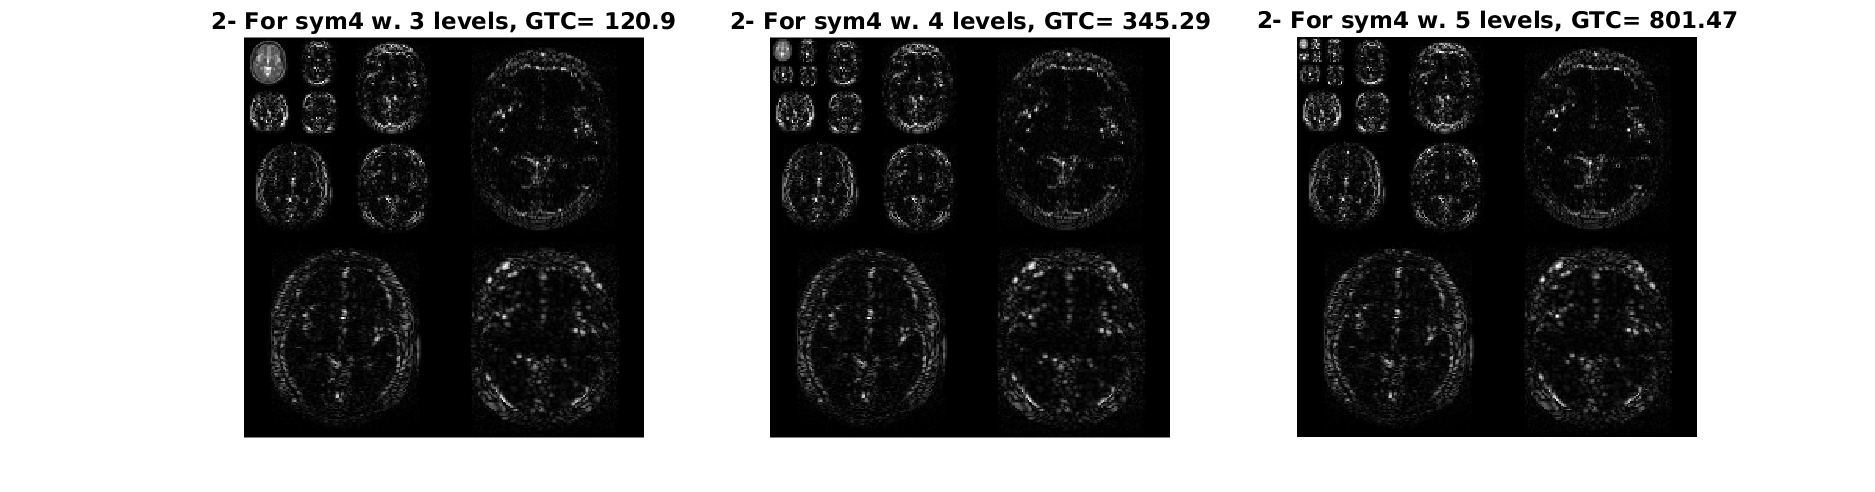
\includegraphics[scale=0.55]{../2_sym4.png}
		\caption{Decomposição usando sym4 para a imagem 2}
	\end{center}
\end{figure}  

\begin{figure}[H]
	\begin{center}
		\label{fig:2_bior3.1}
		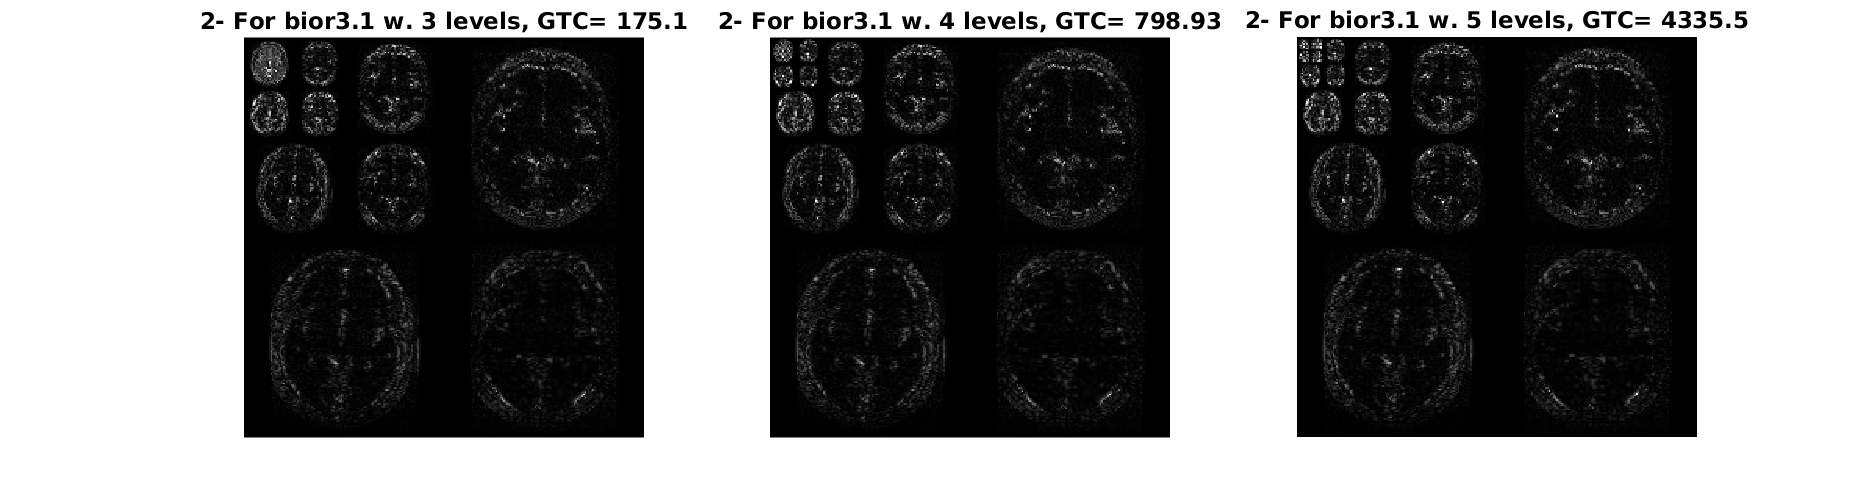
\includegraphics[scale=0.55]{../2_bior31.png}
		\caption{Decomposição usando bior3.1 para a imagem 2}
	\end{center}
\end{figure}  

\subsection*{B - Compressão de Imagens: SNR vs. NM\%}
Baseado no $G_{TC}$ obtido para as decomposições em diferentes níveis foi considerado que a escolha de 5 níveis seria a melhor. Para a implementação computacional foi utilizada a seguinte rotina implementada em MATLAB:

\lstinputlisting[style=Matlab-editor]{../dwt2dQuantizer.m}

Já para o procedimento de reconstrução foi implementado outra rotina para o procedimento reverso que encapsula a função de reconstrução do QMF-2D.

\lstinputlisting[style=Matlab-editor]{../dwt2dReconstruction.m}

\subsection*{C - Comparativo de Resultados}
As imagens \ref{fig:Q1_b_im1} e \ref{fig:Q1_b_im2} apresentam os resultados para as curvas de Taxa vs. Distorção. Nota-se que com a utilização das diferentes wavelets levou a diferentes resultados de performance. Em especial, para a biortogonal houve um ponto de mudança brusca na qual a adição de coeficientes levou ao melhor desempenho para todas as curvas. Em distorções maiores, a sym4 obteve melhor desempenho porém todas as curvas estão bastante próximas para os pontos considerados. 

\begin{figure}[H]
	\begin{center}
		\label{fig:Q1_b_im1}
		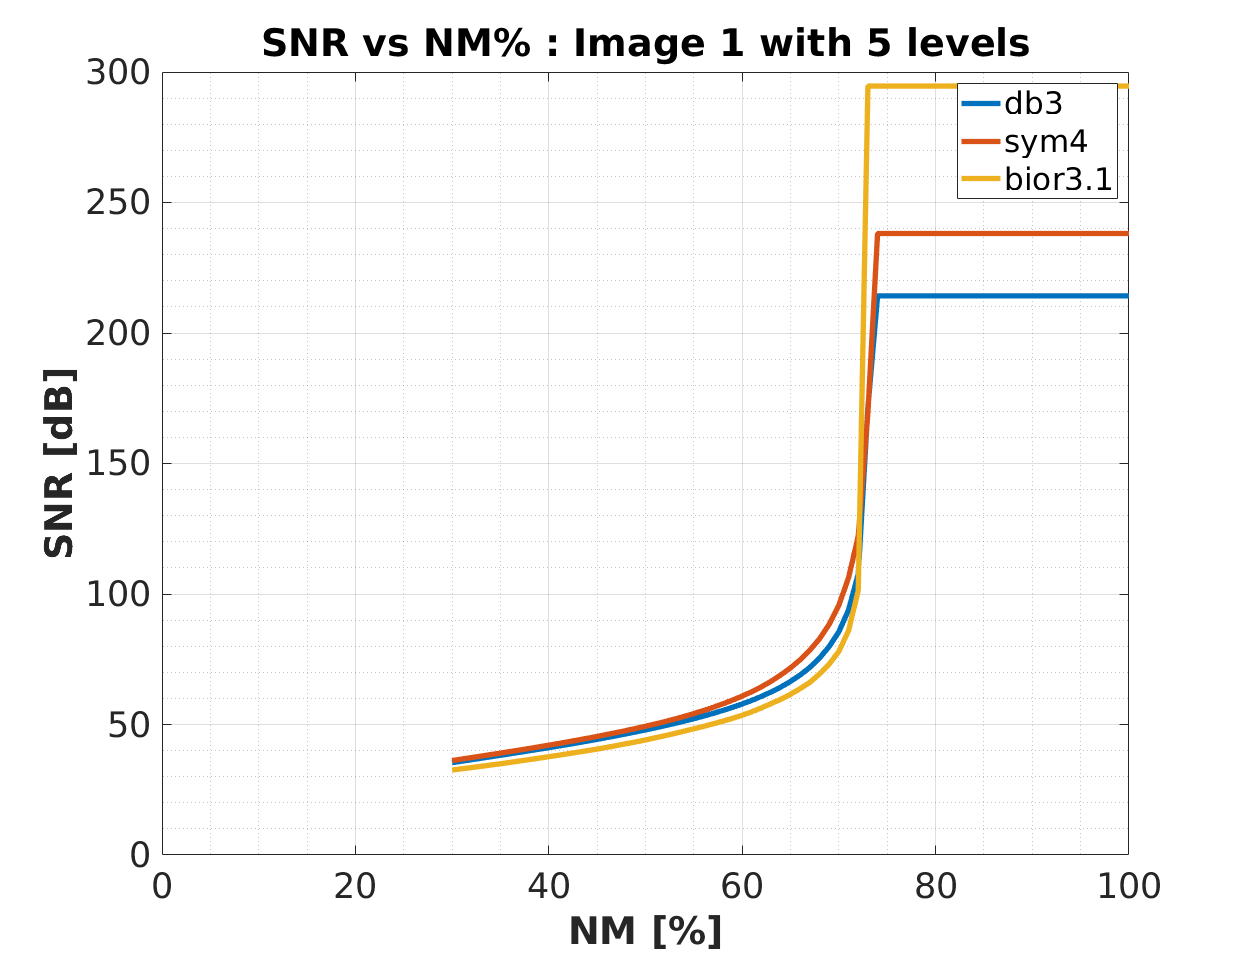
\includegraphics[scale=0.35]{../Q1_b_im1.png}
		\caption{Curva SNR vs. NM\% para a imagem 1}
	\end{center}
\end{figure}  

\begin{figure}[H]
	\begin{center}
		\label{fig:Q1_b_im2}
		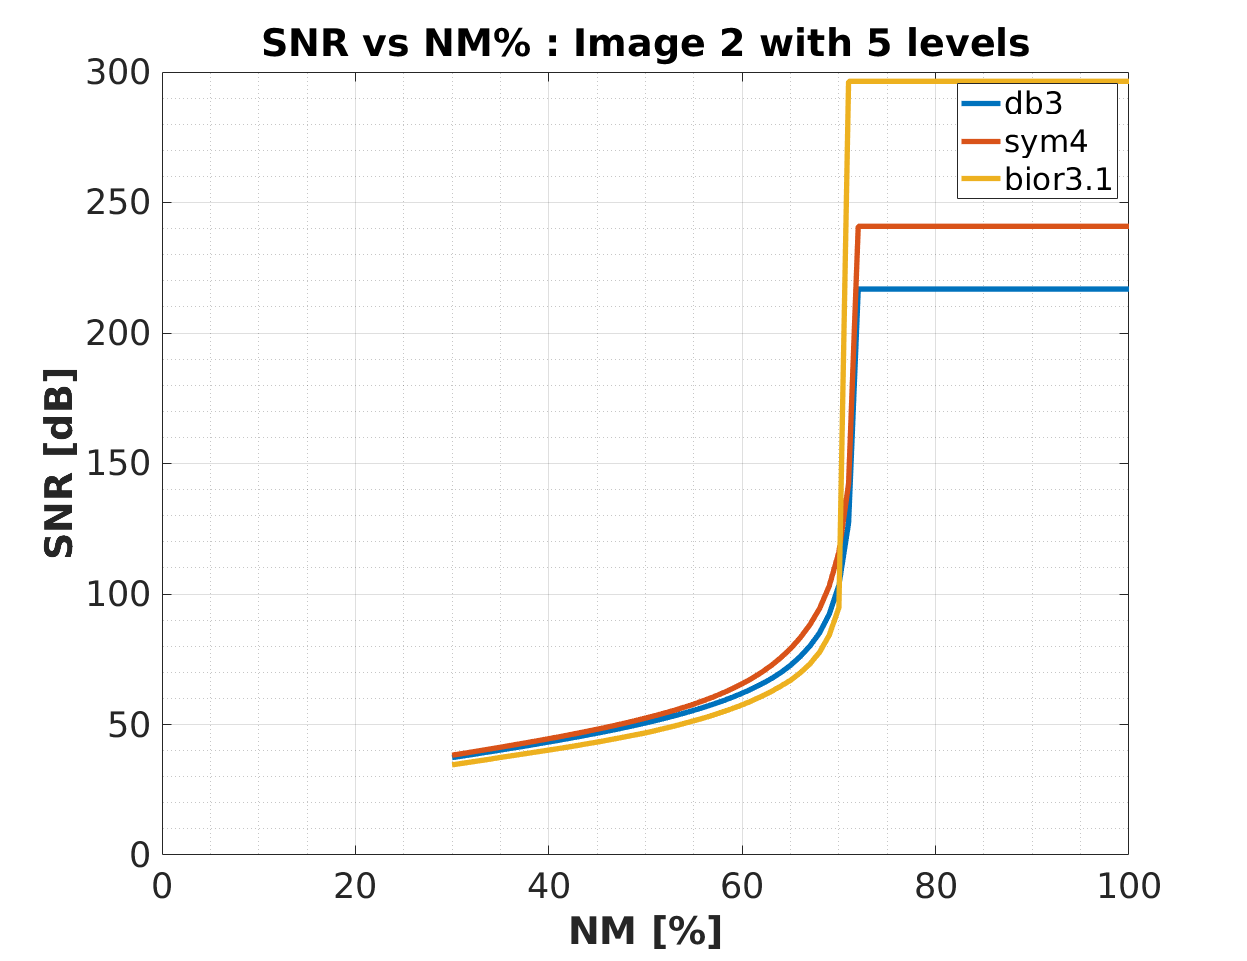
\includegraphics[scale=0.35]{../Q1_b_im2.png}
		\caption{Curva SNR vs. NM\% para a imagem 2}
	\end{center}
\end{figure}  
% --------------------------------------------------------------------------
\section*{Questão 2 - Detecção \& Classificação de Complexos QRS em sinais de ECG}
\subsection*{A - Implementação para detecção QRS}
Baseado na implementação do algoritmo Pan-Tompkins ~\cite{pan}, formulei uma série de simplificações e escolhas que guiaram o desenvolvimento do algoritmo. Inicialmente, realiza-se uma filtragem passa-banda entre 0.5 e 18 Hz com filtro de butterworth (\textit{zero-phase}) para então aplicar o filtro derivativo usado no célebre trabalho original de Pan-Tompkins com 2 amostras de atraso. Posteriormente, a saída do filtro derivativo é elevada ao quadrado para ressaltar conteúdos de alta frequência presentes e é aplicado então uma média-móvel de 85 ms de duração. Com o resultado são detectados picos que estejam com distância miníma de 200 ms entre si já que está é uma condição fisiológica para o sinal considerado e são filtrados picos com valores menores que um limiar relativo a média do sinal integrado. Dessa maneira, é possível localizar bem os pontos R presentes no sinal filtrado sem que ondas acentuadas do tipo T sejam, por vezes, detectadas. Finalmente, realiza-se um refinamento dos picos R usando como referência o sinal original para que as marcações sejam efetivas. Ademais, para os pontos Q e S foram considerados os mínimos locais adjacente ao pico R obtido. Embora simples, a rotina de detecção dos pontos Q e S obteve bons resultados conforme as figuras a seguir. 

Em todos os casos exceto o apresentado na figura ~\ref{fig:qrs_108m3} há resultados condizentes e adequatos para as anotações mostradas. No caso em que há erros o sinal apresenta inversões do pico R seguidas de picos agudos os quais foram errôneamente classificados como picos R. Para situação enunciada a marcação dos pontos Q e S também foi errônea.

\begin{figure}[H]
	\begin{center}
		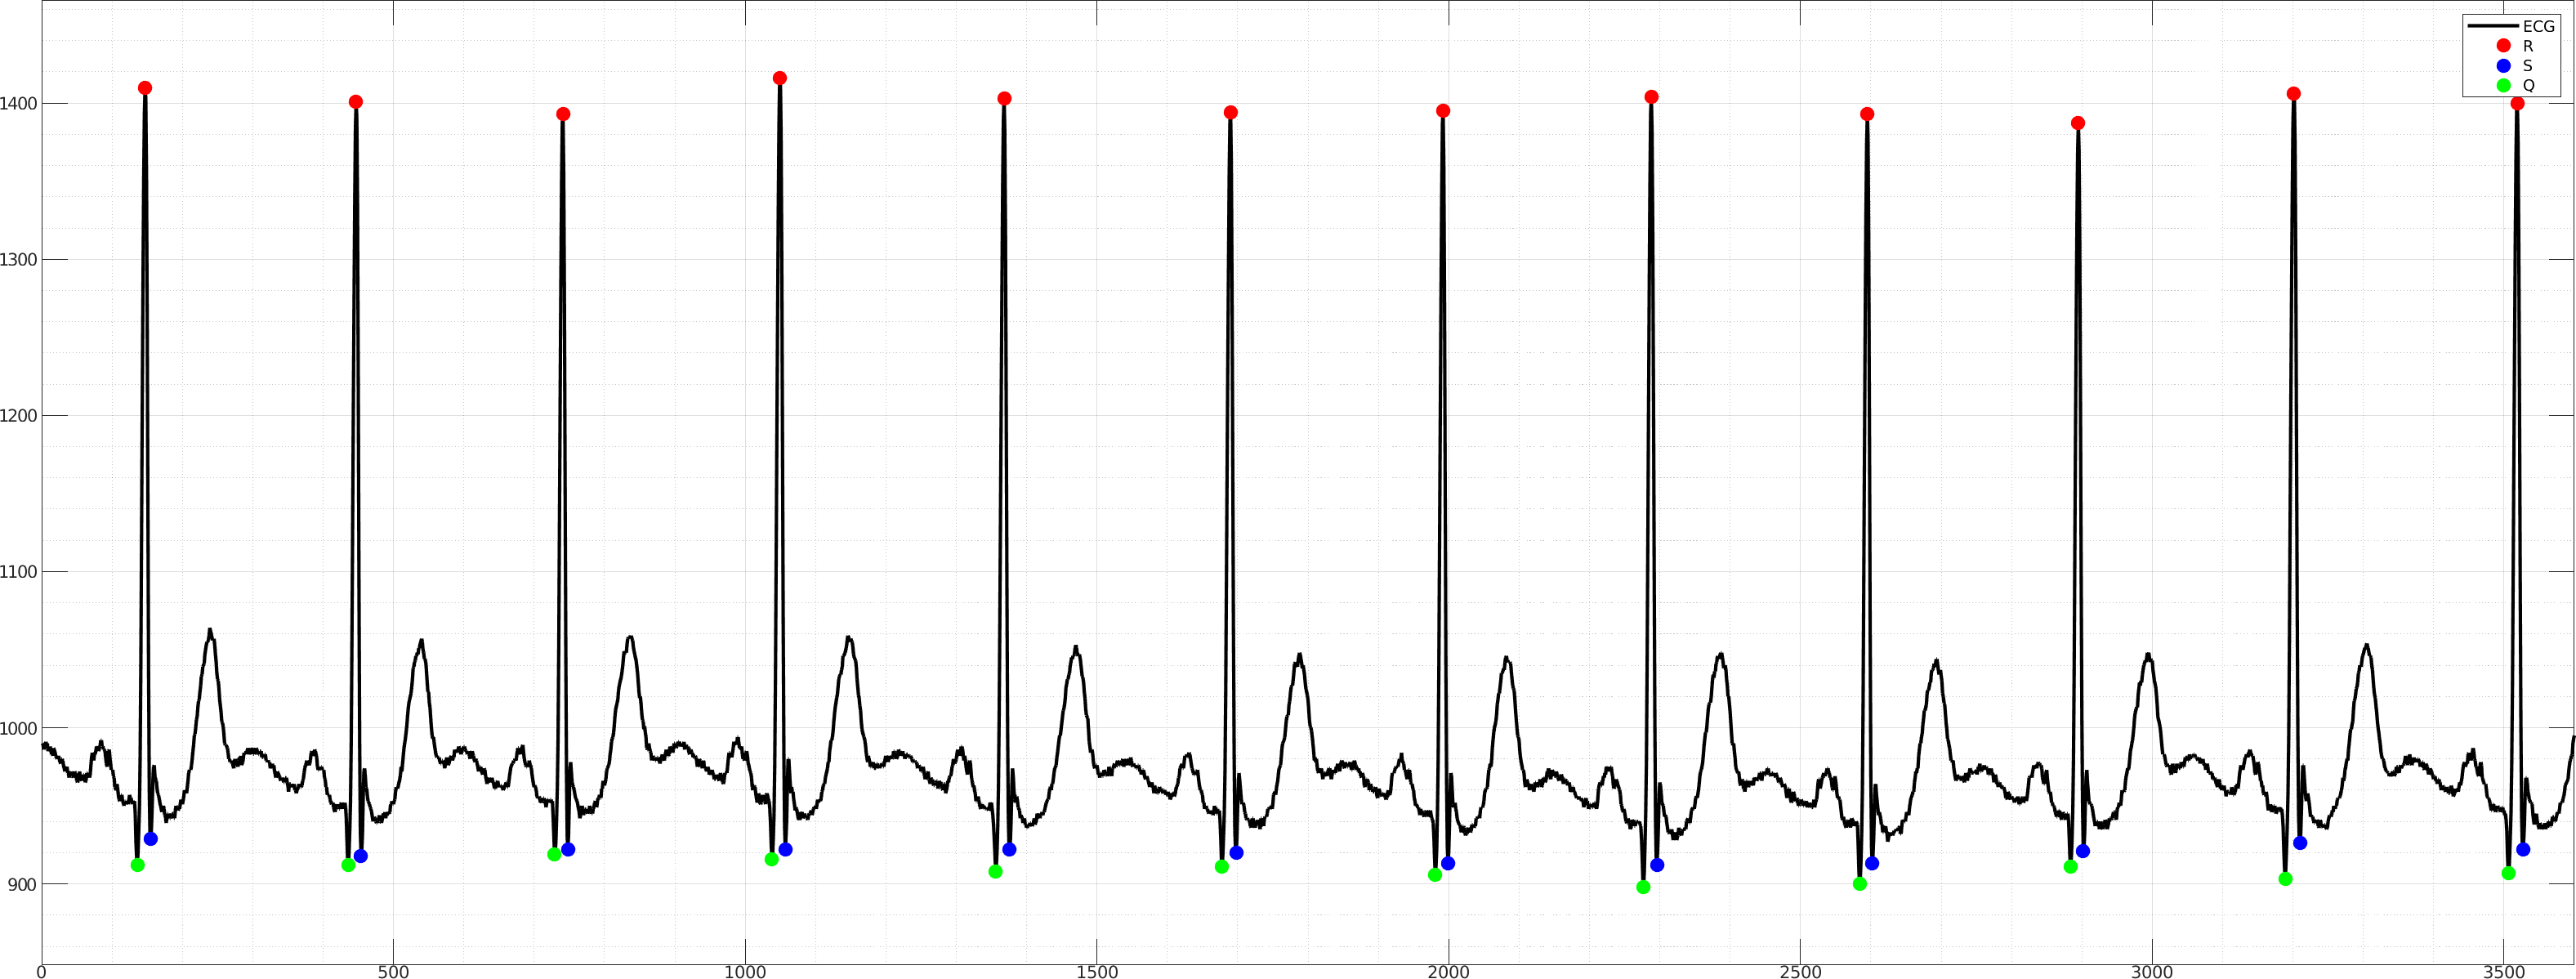
\includegraphics[scale=0.3]{../qrs_103m6.png}
		\caption{Anotações obtidas para o sinal 103m6}
		\label{fig:qrs_103m6}
	\end{center}
\end{figure}  

\begin{figure}[H]
	\begin{center}
		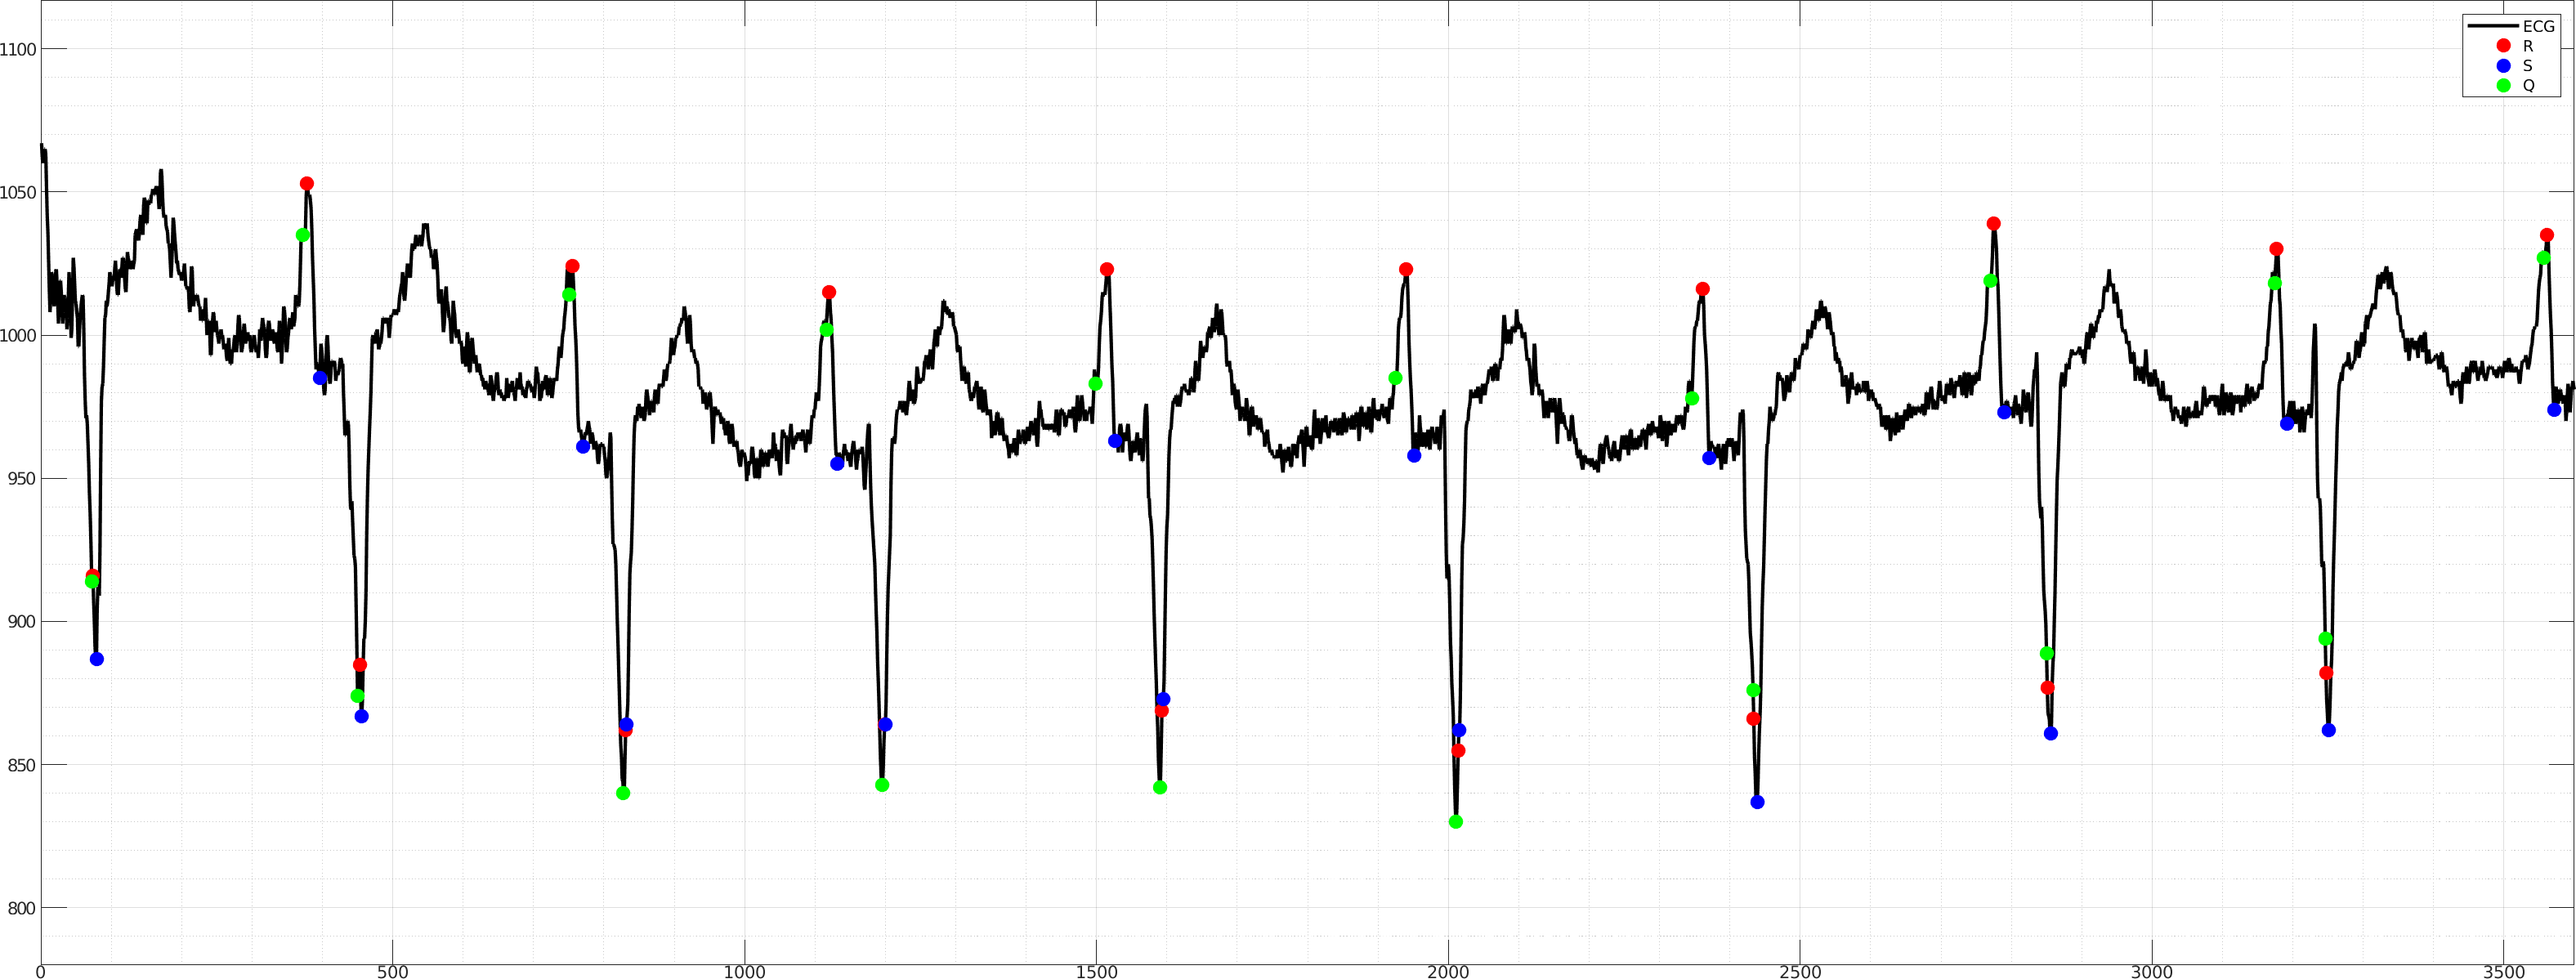
\includegraphics[scale=0.28]{../qrs_108m3.png}
		\caption{Anotações obtidas para o sinal 108m3}
		\label{fig:qrs_108m3}
	\end{center}
\end{figure}  

\begin{figure}[H]
	\begin{center}
		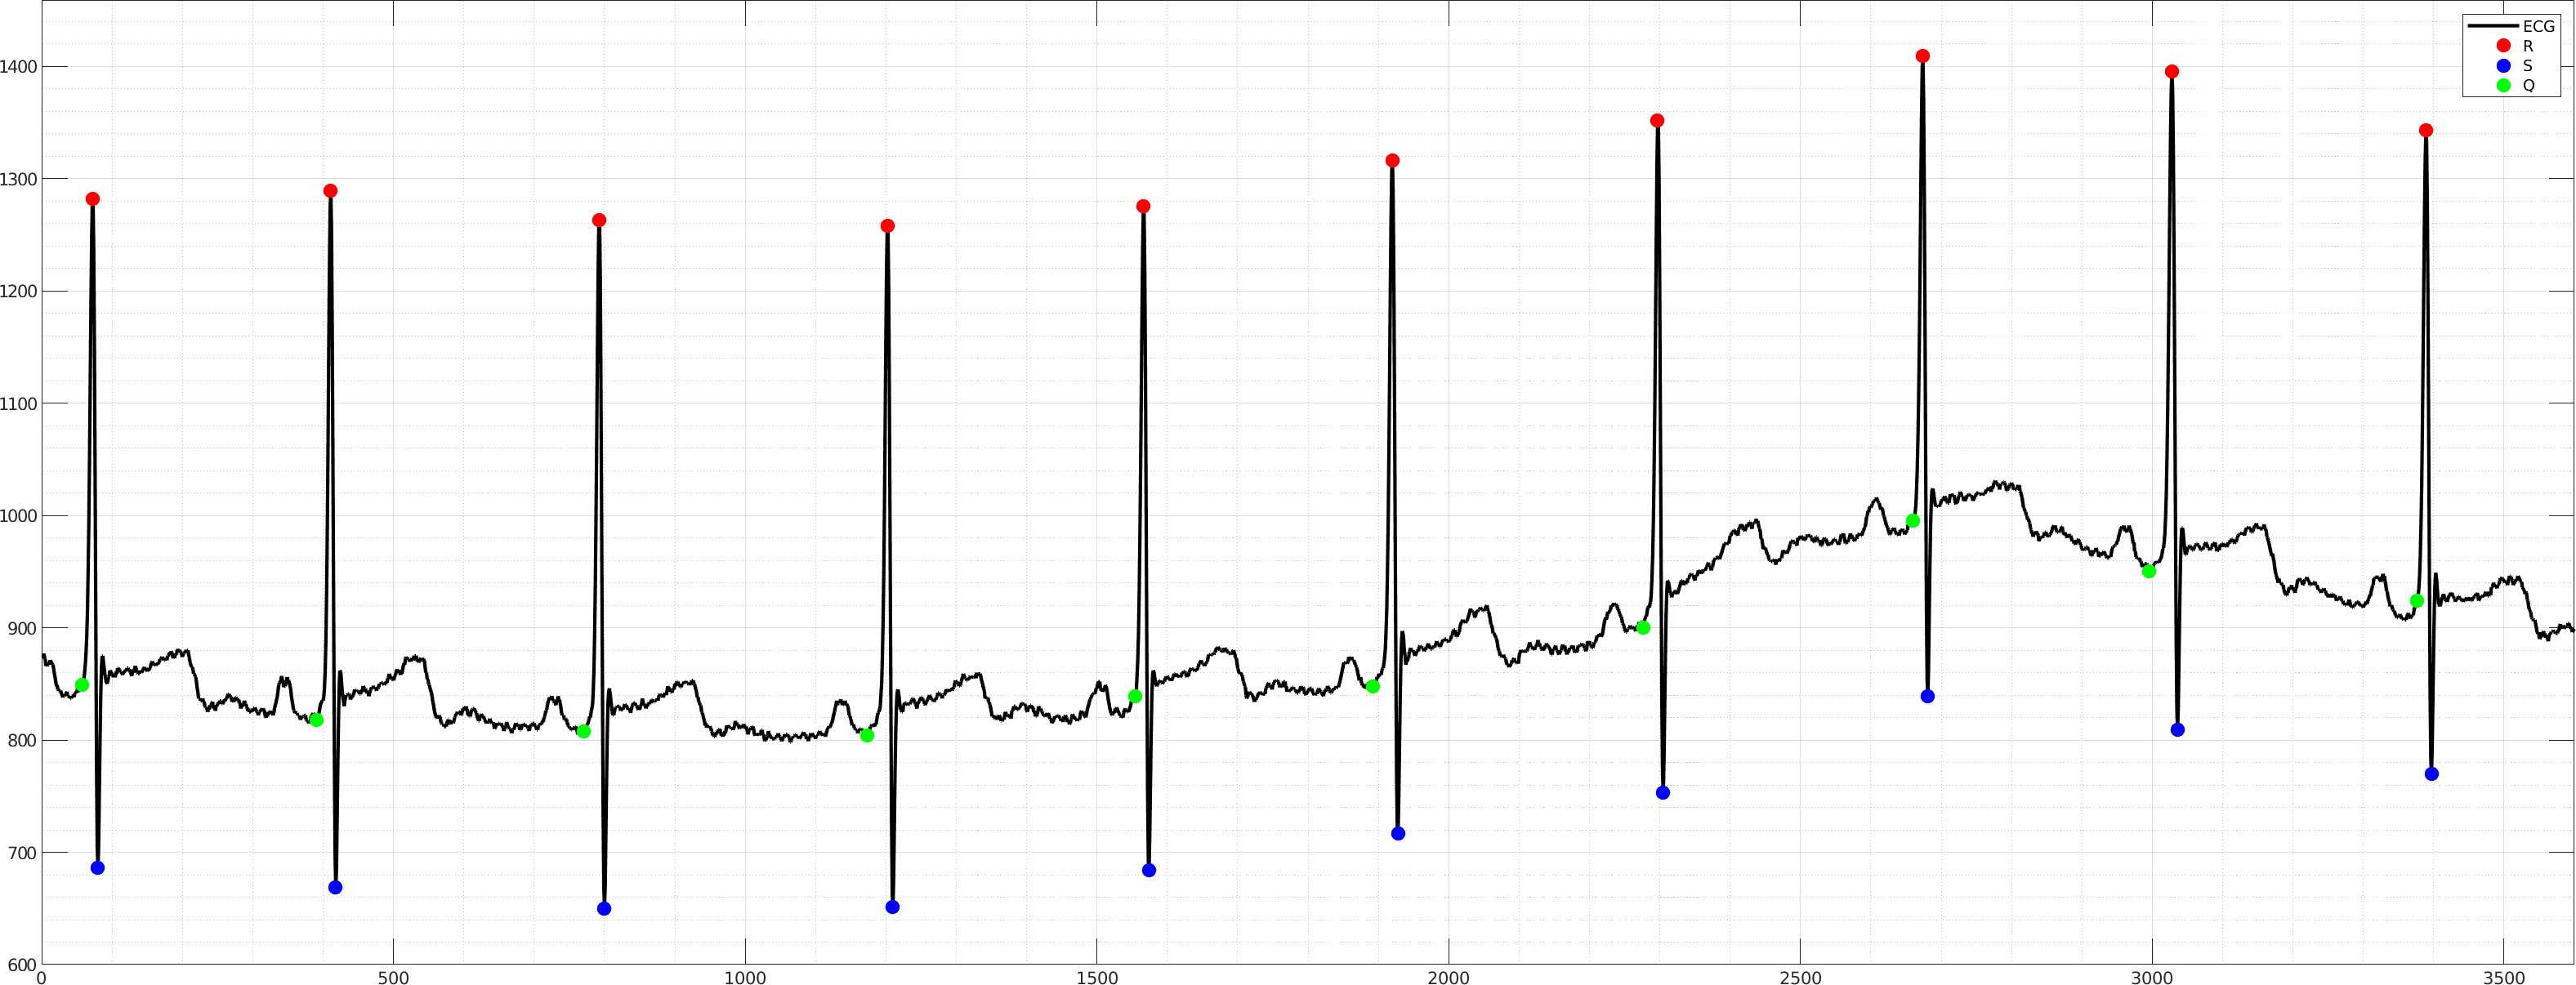
\includegraphics[scale=0.28]{../qrs_115m6.png}
		\caption{Anotações obtidas para o sinal 115m6}
		\label{fig:qrs_115m6}
	\end{center}
\end{figure}  

\begin{figure}[H]
	\begin{center}
		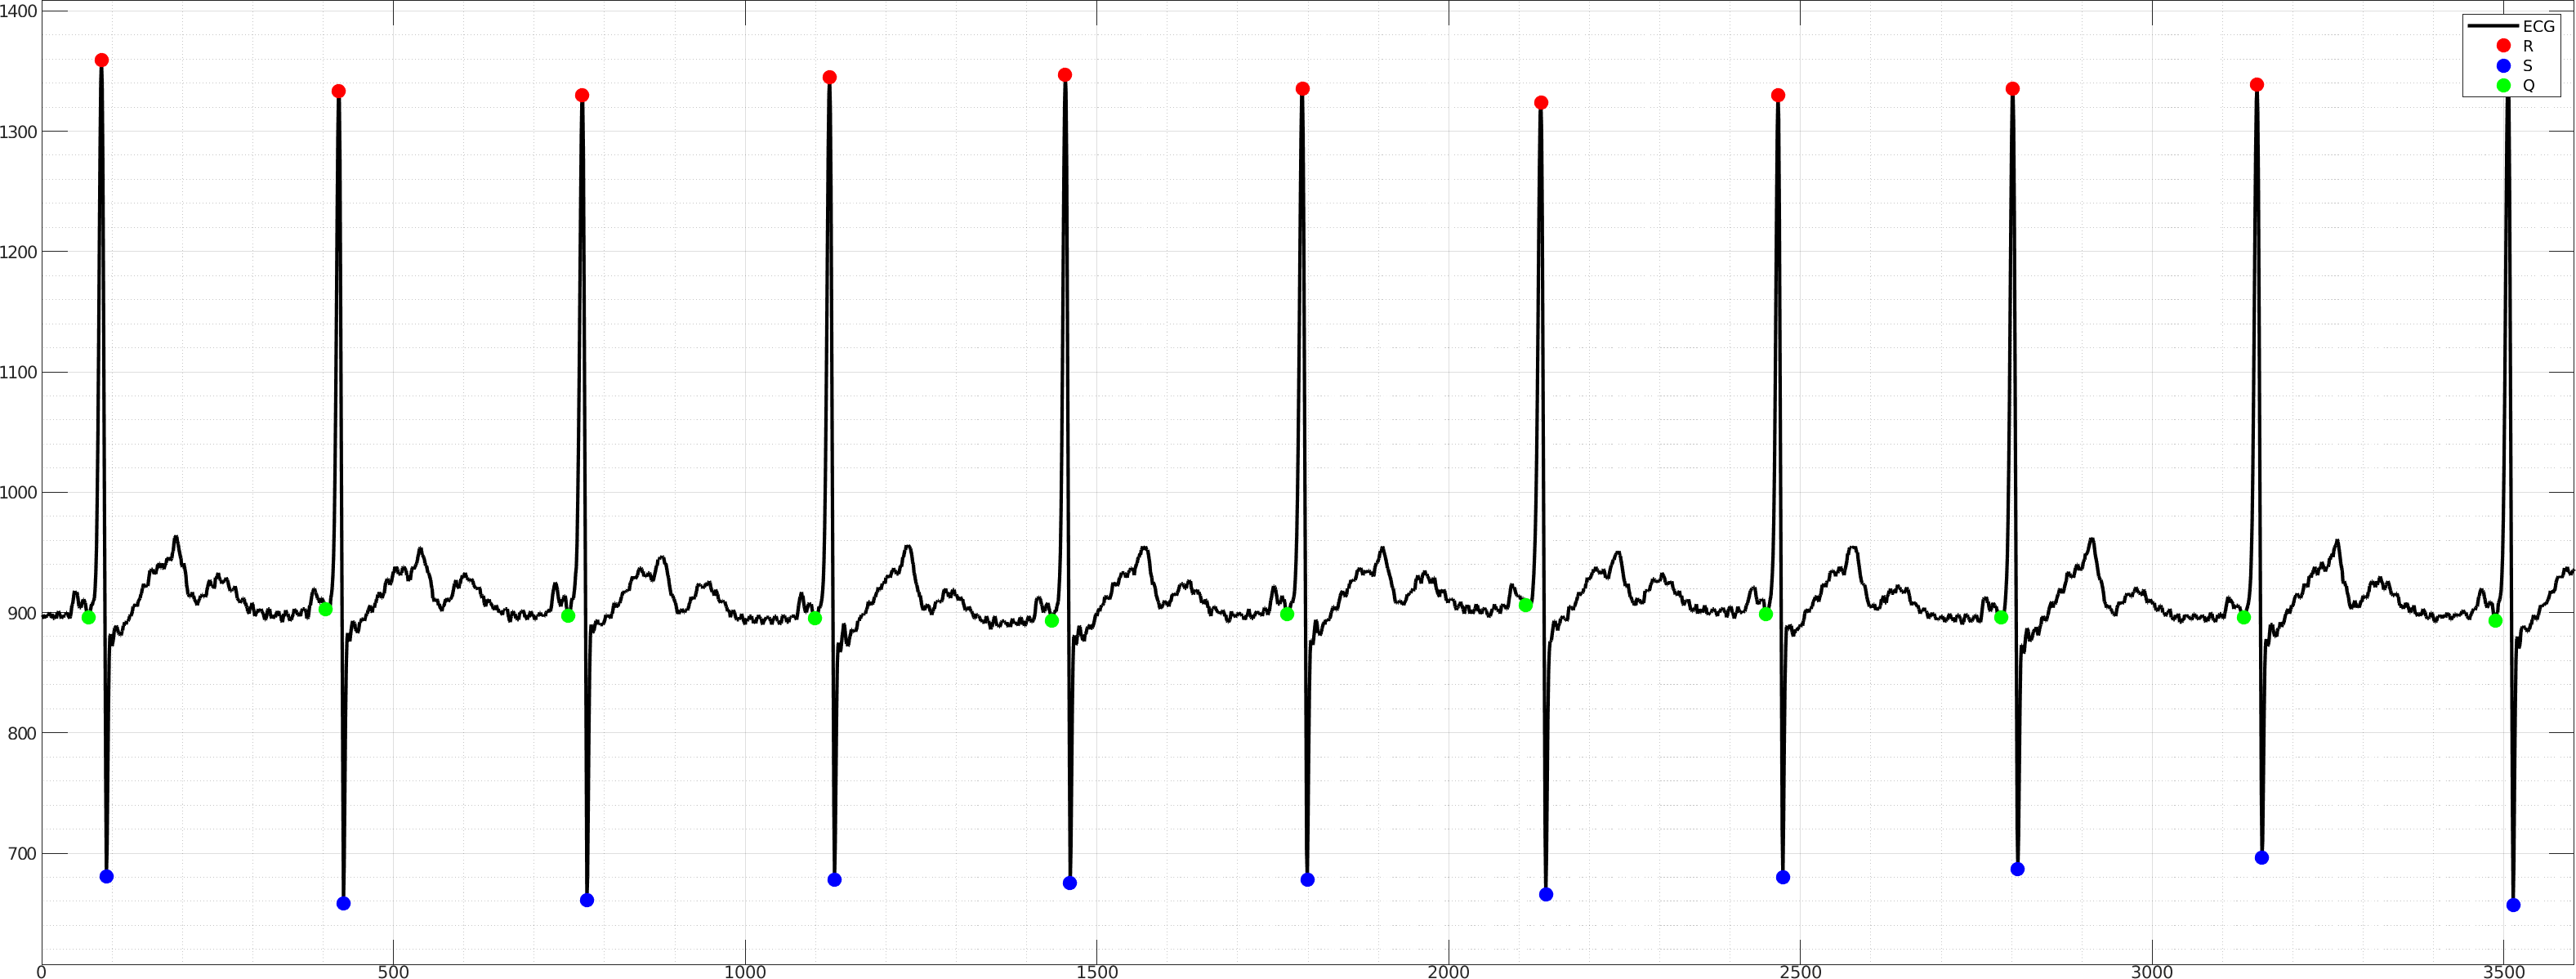
\includegraphics[scale=0.28]{../qrs_220m3.png}
		\caption{Anotações obtidas para o sinal 220m3}
		\label{fig:qrs_220m3}
	\end{center}
\end{figure}  

\begin{figure}[H]
	\begin{center}
		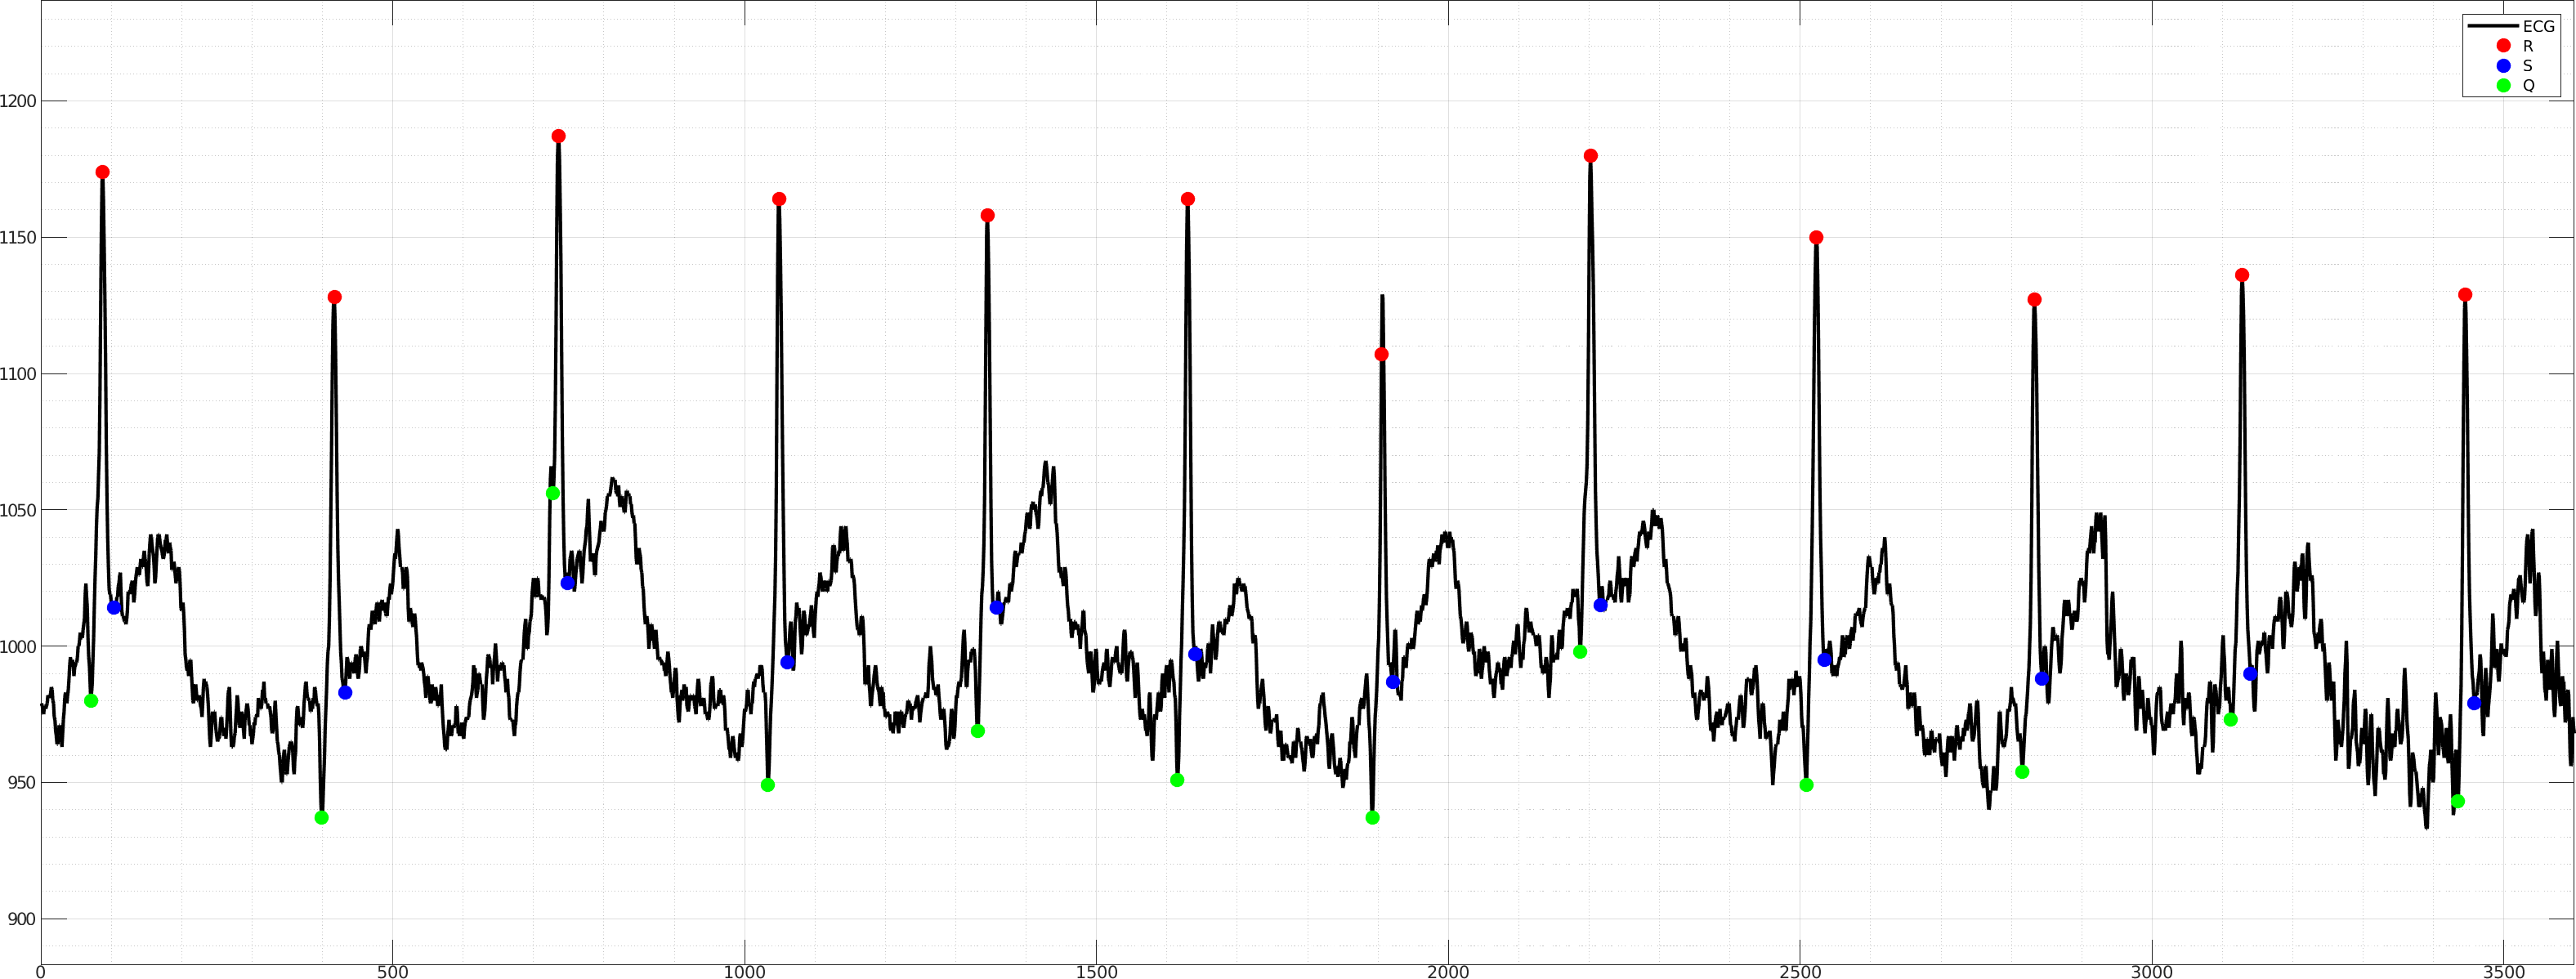
\includegraphics[scale=0.3]{../qrs_228m1.png}
		\caption{Anotações obtidas para o sinal 228m1}
		\label{fig:qrs_228m1}
	\end{center}
\end{figure}  

A implementação segue a seguinte rotina:
\lstinputlisting[style=Matlab-editor]{../rwave_detect.m}

Para os pontos Q e S:
\lstinputlisting[style=Matlab-editor]{../qswave_detect.m}
\newpage
\subsection*{C - Classificação de QRS com SVM}
As tentativas iniciais revelaram que a utilização de \textit{kernel} polinomial ou RBF (\textit{Radial Basis Function}) para as condições de teste geravam excessivo \textit{overfitting} no classificador. Com a utilização de um \textit{kernel} linear foram obtidos resultados interessante com a metodologia de treinamento e validação utilizada.

Para a seleção do conjunto de validação são selecionados 30\% dos sinais de maneira aleatória para extração dos pontos de interesse. O restante dos sinais é utilizado para treinamento de maneira que entre os conjuntos de validação e treinamento não existam dados em comum. Para aumentar a ocorrência de casos positivos no conjunto de treinamento foi utilizado uma sobreposição de 50\% entre as janelas. Como tolerância para o centro da janela foi escolhida uma distância de 40 amostras (11.1 ms). A entrada da SVM recebe janelas de 1 segundo de duração. Ademais, não houve sobreposição de janelas nas condições de validação, algo que gerou poucos casos positivos no conjunto de validação.

Novamente, para reduzir a possibilidade de \textit{overfitting} no modelo foi atribuido um Custo de 8 para falsos negativos e 1 para falsos positivos já que existem bem menos casos positivos que negativos é desejado que, em detrimento de falsos positivos, o classificador não obtenha falsos negativos durante o processo de detecção.

Foram testados cada um dos picos Q, R e S em sessão única de treinamento e validação e os resultados obtidos são mostrados nas figuras a seguir. É válido ressaltar que para todas as métricas mostradas de \textit{FP-Rate} o valor elevado é decorrente do pequeno conjunto de casos positivos já que não foi realizado overlap na validação. Isso é notório pelo fato de que TP-Rate ainda se mantém elevado.

\begin{figure}[H]
	\begin{center}
		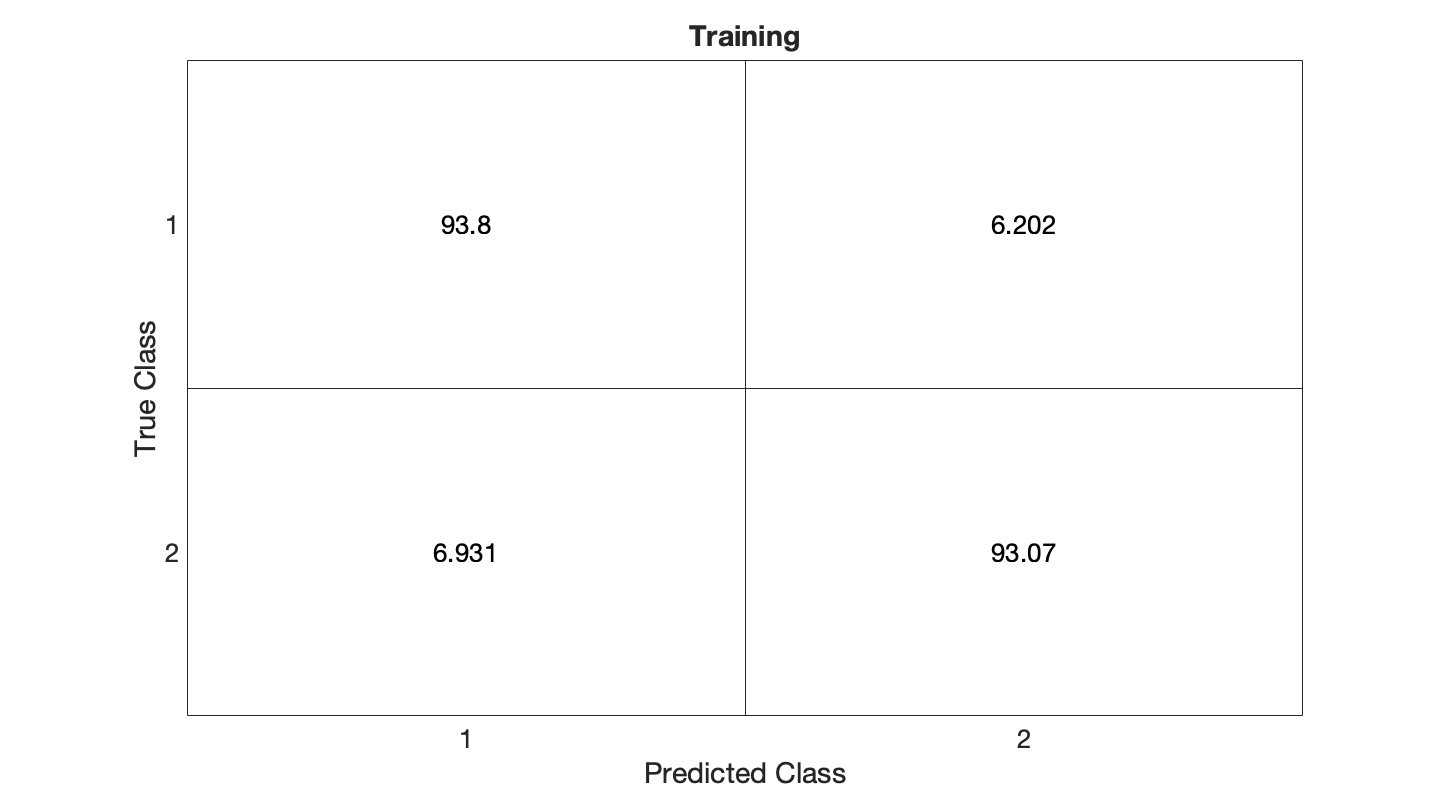
\includegraphics[scale=0.19]{../SVM_train.png}
		\caption{Matriz de Confusão para Treinamento da Classificação do Pico R (valores percentuais)}
		\label{fig:SVM_train}
	\end{center}
\end{figure}  


\begin{figure}[H]
	\begin{center}
		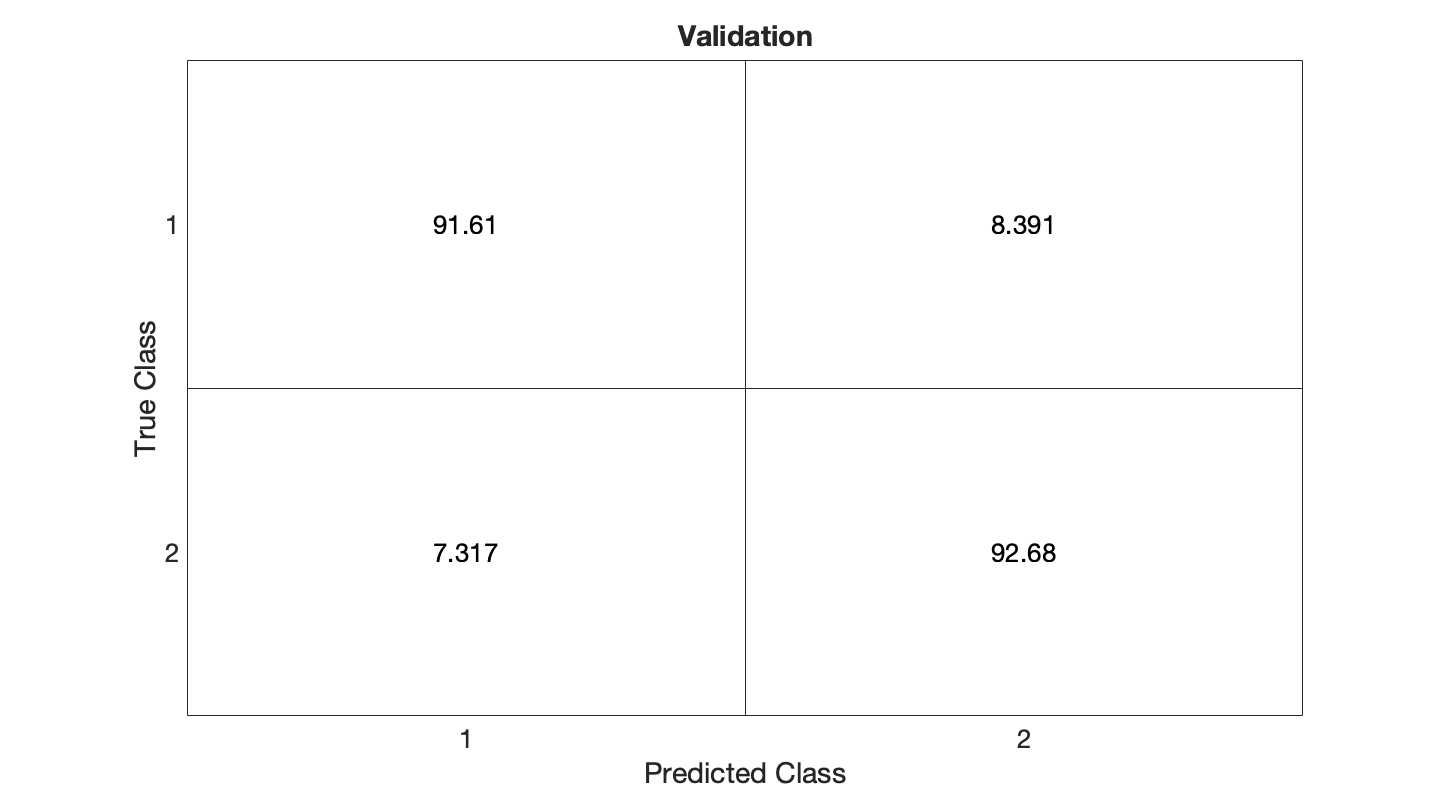
\includegraphics[scale=0.19]{../SVM_val.png}
		\caption{Matriz de Confusão para Validação da Classificação do Pico R (valores percentuais)}
		\label{fig:SVM_val}
	\end{center}
\end{figure}  

\begin{figure}[H]
	\begin{center}
		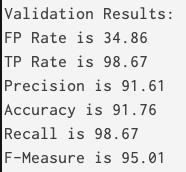
\includegraphics[scale=0.7]{../SVM_metrics.png}
		\caption{Métricas para a sessão de Validação do Pico R}
		\label{fig:SVM_metrics}
	\end{center}
\end{figure}  

\begin{figure}[H]
	\begin{center}
		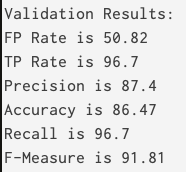
\includegraphics[scale=0.7]{../SVM_q_metrics.png}
		\caption{Métricas para a sessão de Validação do Pico Q}
		\label{fig:SVM_q_metrics}
	\end{center}
\end{figure}  

\begin{figure}[H]
	\begin{center}
		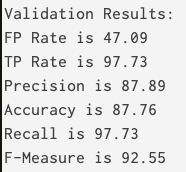
\includegraphics[scale=0.7]{../SVM_s_metrics.png}
		\caption{Métricas para a sessão de Validação do Pico S}
		\label{fig:SVM_s_metrics}
	\end{center}
\end{figure}  
\newpage
\subsection*{D - Detecção de QRS com SVM}
Para a etapa final da detecção utilizei a classificação dos pontos R para a qual foram obtidos melhores resultados. Realizei a marção em algumas janelas e obtive os valores R selecionando pontos de máximo. Como em algum sinais há inversão do pico R, houveram marcações errôneas para o procedimento citado. Abaixo, são exibidas as marcações obtidas (vide figura ~\ref{fig:Q2_d}).

\begin{figure}[H]
	\begin{center}
		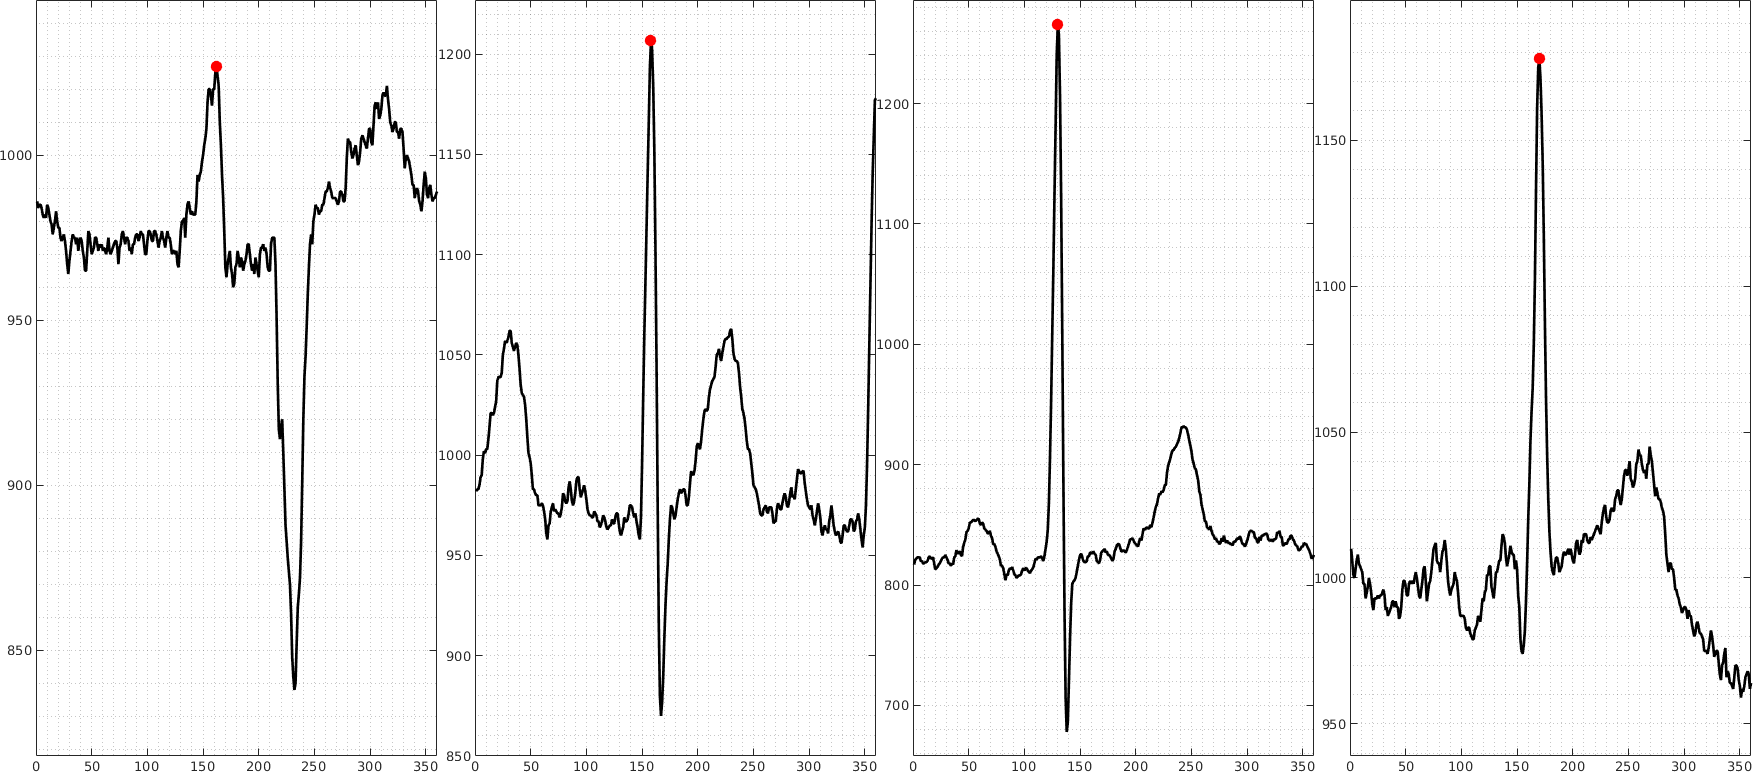
\includegraphics[scale=0.3]{../Q2_d.png}
		\caption{Marcações para o ponto R em diferentes janelas.}
		\label{fig:Q2_d}
	\end{center}
\end{figure}  

\begin{figure}[H]
	\begin{center}
		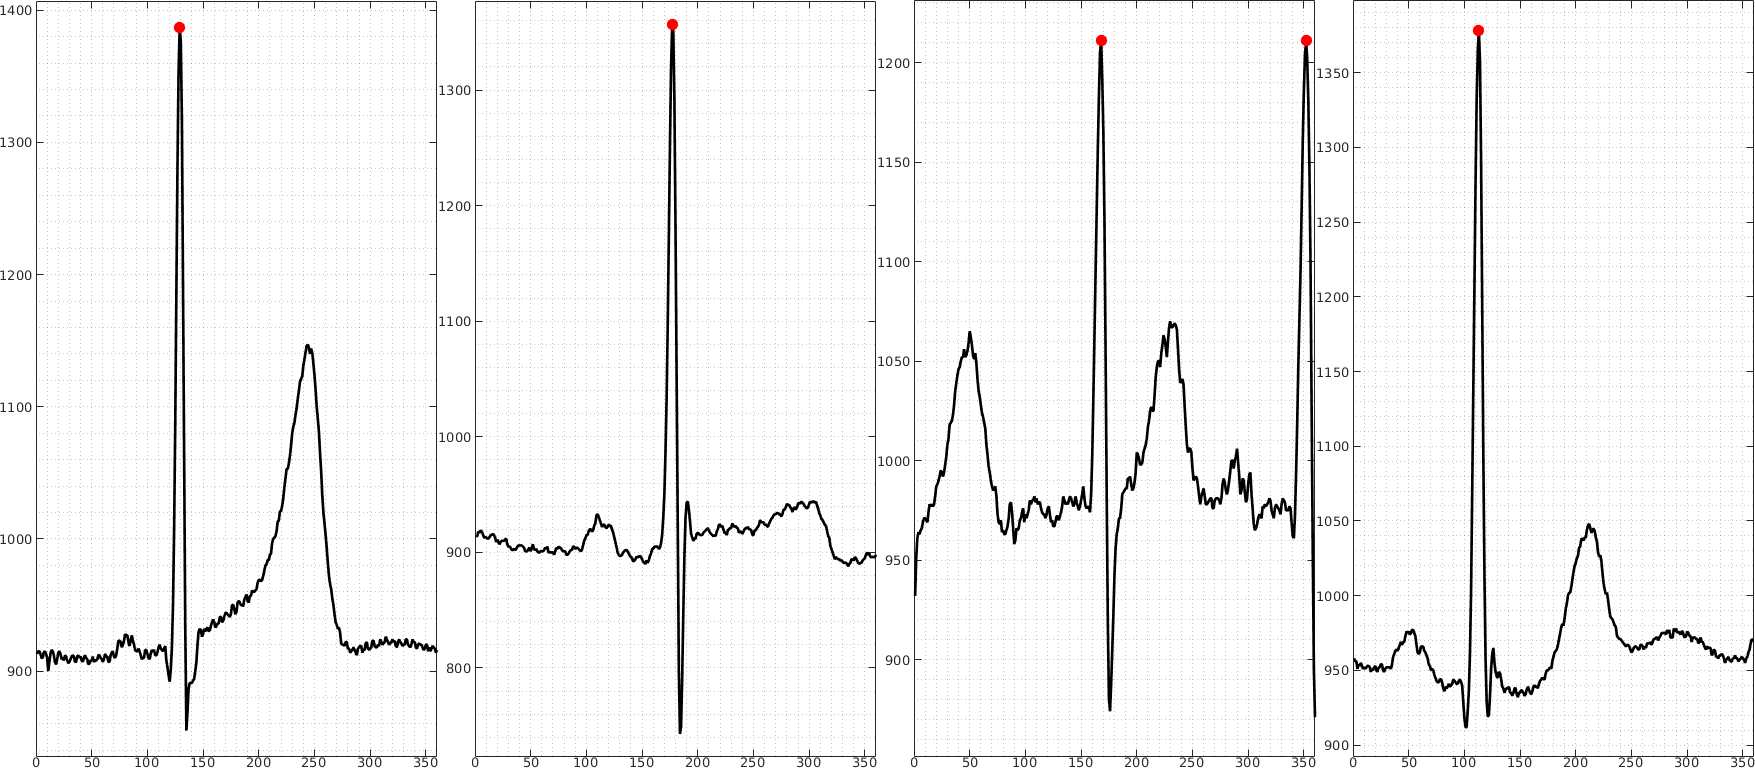
\includegraphics[scale=0.3]{../Q2_d2.png}
		\caption{Marcações para o ponto R em diferentes janelas.}
		\label{fig:Q2_d2}
	\end{center}
\end{figure} 

\newpage
\section*{Considerações Finais}
Considero que o escopo da matéria foi bastante extenso e me possibilitou sistematizar conteúdos e explorar implementações que não havia feito antes e que foram bastante divertidas em sua grande maioria! Além disso, o conteúdo foi cumprido de maneira excepcional já que foi possível esclarecer todos os tópicos que tive dificuldade com o auxílio das aulas presenciais ou por meio dos trabalhos práticos desenvolvidos na prova 1 e 2. Finalmente, agradeço por toda a ajuda prestada ao longo do semestre e pelas aulas.

Muito Obrigado, \textbf{Davi Mendes}.



% --------------------------------------------------------------------------
\begin{thebibliography}{1}
\bibitem{jayant} 
N.S. Jayant, P. Noll, Digital Coding of Waveforms, Prentice-Hall, 1984.
\bibitem{pan}
Pan, J., Tompkins, W.J.: A real-time QRS detection algorithm. IEEE Trans. Biomed. Eng. 3, 230–236 (1985)
\end{thebibliography}

\newpage
\section*{Anexos}
\subsection*{Questão 1 - Implementação completa}
\lstinputlisting[style=Matlab-editor]{../Q1.m}

\subsection*{Questão 2 - Implementação completa}
\lstinputlisting[style=Matlab-editor]{../QRS.m}
\subsection*{Questão 2 - Implementação com SVM}
\lstinputlisting[style=Matlab-editor]{../QRS_svm.m}
% -------------------------------------------------------------------------
\end{document}
